%-----------------------------------------------------------------------------
%
%               Template for sigplanconf LaTeX Class
%
% Name:         sigplanconf-template.tex
%
% Purpose:      A template for sigplanconf.cls, which is a LaTeX 2e class
%               file for SIGPLAN conference proceedings.
%
% Guide:        Refer to "Author's Guide to the ACM SIGPLAN Class,"
%               sigplanconf-guide.pdf
%
% Author:       Paul C. Anagnostopoulos
%               Windfall Software
%               978 371-2316
%               paul@windfall.com
%
% Created:      15 February 2005
%
%-----------------------------------------------------------------------------


%\documentclass[preprint]{sigplanconf}
\documentclass[10pt]{sigplanconf}

% The following \documentclass options may be useful:
%
% 10pt          To set in 10-point type instead of 9-point.
% 11pt          To set in 11-point type instead of 9-point.
% authoryear    To obtain author/year citation style instead of numeric.

\usepackage{yfonts}
\usepackage{amsmath}
\usepackage{amsthm}
\usepackage{amssymb}
%\usepackage{mathpartir}
\usepackage[colorlinks=true,
citecolor=citec,
linkcolor=linkc,
urlcolor=urlc,
]{hyperref}
\usepackage{url}
\usepackage{graphics}
\usepackage{graphicx}
\usepackage{wasysym}
\usepackage{harmony}
\usepackage{marvosym}
\usepackage{multirow}
\usepackage[nameinlink,nosort]{cleveref}
\usepackage{xeCJK}
\usepackage[usenames,dvipsnames]{xcolor}
\usepackage[utopia]{mathdesign}
\usepackage{natbib}
\usepackage{ulem}
\usepackage[mathcal]{euscript}
\usepackage[linesnumbered,ruled]{algorithm2e}

\renewcommand{\UrlBreaks}{\do\/\do\a\do\b\do\c\do\d\do\e\do\f\do\g\do\h\do\i\do\j\do\k\do\l\do\m\do\n\do\o\do\p\do\q\do\r\do\s\do\t\do\u\do\v\do\w\do\x\do\y\do\z}


% ____________________________________________________________
% Listings Package Configuration
% \usepackage[scaled]{beramono}

%\renewcommand*\ttdefault{txtt}
\usepackage[T1]{fontenc}

\definecolor{citec}{RGB}{128,0,64}
\definecolor{linkc}{RGB}{0,64,128}
\definecolor{urlc} {RGB}{128,64,0}

\setCJKmainfont{HeiseiMinStd-W5}[Path = ./]
% This Deep Tex Voodoo is from
%   <http://www.latex-community.org/forum/viewtopic.php?f=5&t=2072>
% It's purpose is to make \lstinline normal size, without affecting
% \lstinputlisting.  It seems to work but I have no idea how or why,
% and I rather hope never to learn.
%\makeatletter
%\lst@AddToHook{TextStyle}{\let\lst@basicstyle\ttfamily\normalsize}
%\makeatother

\begin{document}

\conferenceinfo{SIGBOVIK '19}{Pittsburgh, PA, USA}
\copyrightyear{2019}
\copyrightdata{}

\titlebanner{banner above paper title}        % These are ignored unless
\preprintfooter{short description of paper}   % 'preprint' option specified.

\title{
Which ITG Stepcharts are Bracket-Jumpiest?: \\
In Which They Milk the \\
「A Boring Follow-Up Paper to \\
``Which ITG Stepcharts are Turniest?'' \\
Titled, ``Which ITG Stepcharts are Crossoveriest and/or Footswitchiest?''」\\
Series for All Its Worth in Publication Count After All \\
%That `Boring' Stuff Was Part of the Title, BTW. \\
%So was that. And that, and this too. \\
%You got it all, right? \\
%Or Just, ``More Boring Crap about ITG'', for Short. \\
%Oh, That Was Also Part of the Title.
}
% \subtitle{\em The Randomly-Scoped Lambda Calculus}
% \subtitle{Subtitle Text, if any}

\authorinfo{Ben Blum}{}{bblum@alumni.cmu.edu}

\maketitle

\begin{abstract}
	%ITG is a popular dance game in which players step on arrows while listening to music. The arrow patterns, indicated by a {\em stepchart}, may range among any level of complexity and difficulty. Among the many factors contributing to a stepchart's difficulty is how much the player must turn from side to side.
	%Other more obvious factors, such as raw speed, have been well studied in prior work.
	%This paper presents an analytic study of this {\em turniness} factor.
	%We study the turniness of many existing stepcharts, and present a novel (but unsurprising) approach to automatically generating maximally (or minimally) turny charts.
	%Among real-world songs, we find stepcharts with overall turniness ranging from 0\% to 81.33\% of the theoretical maximum.

In which I break last last year's promise of no future work.

\end{abstract}

\category{D.D.R.}{Exercise and Fitness}{Arcade Dance Games}

\keywords
bracket, groove, in, jumps, the


\section{Introduction}

Recent work by \cite{dril}
%[W. Dril et al., 2019]
proposed the hypothesis that
recent stepchart authors have grown bored with the array of technical ITG step patterns
documented to date \cite{turniness,crossoveriness},
and have moved on to break the old model's one-foot-per-arrow assumption to allow for even more technical patterns yet.
I paraphrase their main conclusion as follows:

\begin{center}
	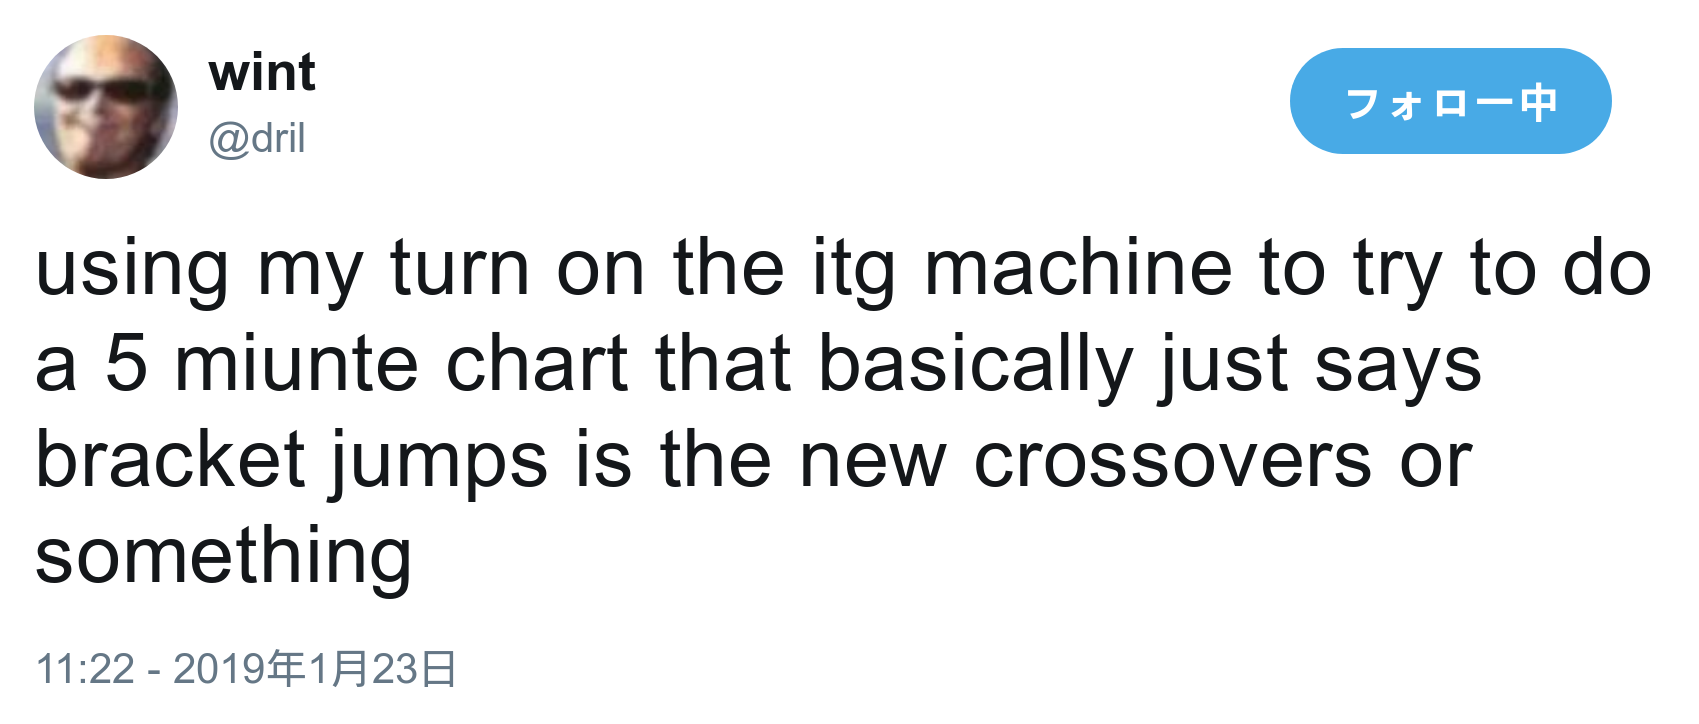
\includegraphics[width=0.42\textwidth]{using-my-turn.png}
\end{center}

All good researchers know that when rise the standards for software or hardware performance
(or stepchart trickiness, as the case may be),
they must revisit their own work to prove its ongoing relevance to the research (dance) community at large.
Thus I must regrettably break the promise \sout{I} the authors set forth in \cite{crossoveriness}
(see \Cref{fig:you-stutid-fuckass})
and revisit \sout{my} their old future work section
(XXX: they said to change any first-person ``our prior work''
stuff like this for double-blind review but like cmon this makes no sense?
theyll totally see through this
(TODO: maybe email the PC chair for advice?
(FIXME: make sure to remove these comments before the camera-ready deadline!!))),
extending it to handle these new so-called ``bracket'' jumps.

\begin{figure}[t]
	\hspace{-2em}\includegraphics[angle=270,width=0.54\textwidth]{../2/paper.pdf}
	\caption{(yeah i reused this joke from last time ok deal)}
	\label{fig:you-stutid-fuckass}
\end{figure}

%%%%%%%%%%%%%%%%%%%%%%%%%%%%%%%%%%%%%%%%%%%%%%%%%%%%%%%%%%%%%%%%%%%%%%%%%%%%%%%%

\section{Overview}

% TODO: go through this paper and make every *other* instance of "bracket-jump" hyphenated

What, then, is a bracket jump (which I shall \textit{not}, henceforth, abbreviate for brevity)?
Put simply, whenever two arrow-shaped obstacles proceed simultaneously towards the protagonist directional indicator targets
(see \cite{turniness}),
while a novice player might think they must step with both feet at once, one for each arrow,
experts often find it more convenient (i.e., less overall foot motion) to use whichever single foot is closer at the time
to hit both arrows by stepping across the metal bracket enclosing the corners of each panel
(thereby triggering one sensor with the heel and one with the little bitty toesies), hence ``bracket jump''.
In case my verbal explanation is not up to snuff, I have also included in \Cref{fig:how-2-bracket}
a high-quality graphics render of a player's typical foot positions during a down+right bracket jump (henceforth ``DR'', et cetera).

\begin{figure}[h]
	\begin{center}
		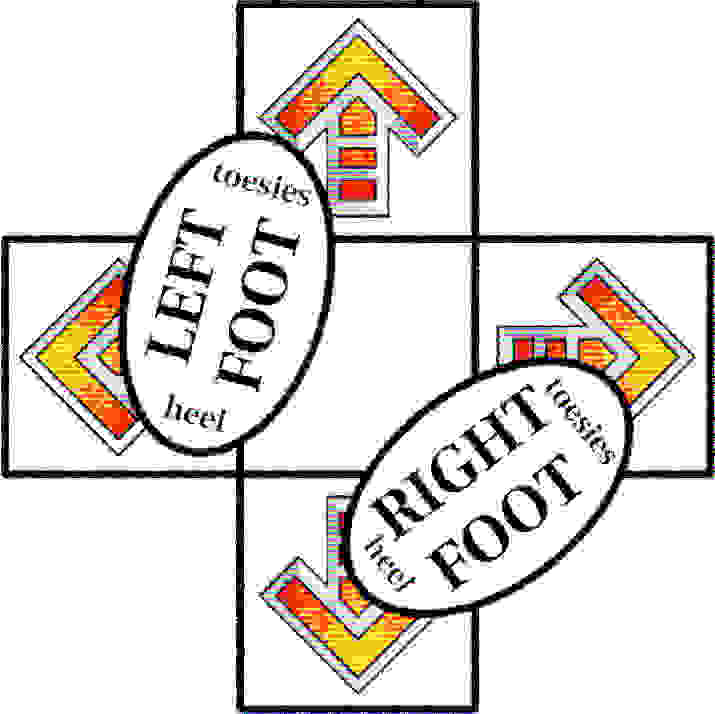
\includegraphics[width=0.48\textwidth]{how-2-bracket.jpg}
	\end{center}
	\caption{Down+right bracket jump real-world example.}
	\label{fig:how-2-bracket}
\end{figure}



%%%%%%%%%%%%%%%%%%%%%%%%%%%%%%%%%%%%%%%%%%%%%%%%%%%%%%%%%%%%%%%%%%%%%%%%%%%%%%%%

\section{Analyzing Bracket-Jumpiness}


%%%%%%%%%%%%%%%%%%%%%%%%%%%%%%%%%%%%%%%%%%%%%%%%%%%%%%%%%%%%%%%%%%%%%%%%%%%%%%%%

\section{Evaluation}


%%%%%%%%%%%%%%%%%%%%%%%%%%%%%%%%%%%%%%%%%%%%%%%%%%%%%%%%%%%%%%%%%%%%%%%%%%%%%%%%

\section{Discussion}

% TODO tings to talk about

% authors seem to know it's easy to overdo -- see, "Stupid" and "I'm sorry" as chart authors in some of the top charts

% many old charts written without regard to jump patterning can be bracker anyway, see OWA (which just makes the list bc it's long)
% - have a figure of OWA in the strema that shows the *non* bracketable stream jumps
% - make a test case that captures these and shows indeed they are not brackets

% temporal analysis of pack age vs bracker density

% other charts of note
% - chicago timing / electrical paradise: bracketiest chart where *ALL* jumps are brackets (BJJ%=100) -- quite tasteful actually!
% - encore is 2nd place lmao

% conclusion: BJJ% is sa better measure of chart funness than BJS%?

\section{Future Work}

It would be cool to integrate this (and the preceding two algorithms \cite{turniness,crossoveriness})
into Simply Love \cite{simplylove}, or whatever the prevailing stepmania theme may be in the future.
Currently, as shown in \Cref{fig:songpreview}, % TODO
the song preview screen wastes considerable space displaying the count of more irrelevant chart aspects
such as mines (now used primarily for signaling the presence of footswitches)
and hands (now mostly stepped with the feet by bracketing anyways).
I bet the community might actually pay attention to my work -- the holy grail of research, honestly --
if the premier dance game theme could tell precisely how technical a chart was in such modern terms.

\section{Conclusion}



%%%%%%%%%%%%%%%%%%%%%%%%%%%%%%%%%%%%%%%%%%%%%%%%%%%%%%%%%%%%%%%%%%%%%%%%%%%%%%%%

\bibliographystyle{abbrvnat}
\bibliography{citations}

\end{document}
